\documentclass{article}
\usepackage{float}

%%%%%%%%%%%%%%%%%%%%%%%%%%%%%%%%%%%%%%%%%
% Lachaise Assignment
% Structure Specification File
% Version 1.0 (26/6/2018)
%
% This template originates from:
% http://www.LaTeXTemplates.com
%
% Authors:
% Marion Lachaise & François Févotte
% Vel (vel@LaTeXTemplates.com)
%
% License:
% CC BY-NC-SA 3.0 (http://creativecommons.org/licenses/by-nc-sa/3.0/)
% 
%%%%%%%%%%%%%%%%%%%%%%%%%%%%%%%%%%%%%%%%%

%----------------------------------------------------------------------------------------
%	PACKAGES AND OTHER DOCUMENT CONFIGURATIONS
%----------------------------------------------------------------------------------------

\usepackage{amsmath,amsfonts,stmaryrd,amssymb} % Math packages

\usepackage{enumerate} % Custom item numbers for enumerations

\usepackage[ruled]{algorithm2e} % Algorithms

\usepackage[framemethod=tikz]{mdframed} % Allows defining custom boxed/framed environments

\usepackage{listings} % File listings, with syntax highlighting
\lstset{
	basicstyle=\ttfamily, % Typeset listings in monospace font
}

\usepackage{subfigure}

%----------------------------------------------------------------------------------------
%	DOCUMENT MARGINS
%----------------------------------------------------------------------------------------

\usepackage{geometry} % Required for adjusting page dimensions and margins

\usepackage{setspace}

\onehalfspacing

\geometry{
	paper=a4paper, % Paper size, change to letterpaper for US letter size
	top=3cm, % Top margin
	bottom=3.5cm, % Bottom margin
	left=3cm, % Left margin
	right=3cm, % Right margin
	headheight=14pt, % Header height
	footskip=1.5cm, % Space from the bottom margin to the baseline of the footer
	headsep=1.2cm, % Space from the top margin to the baseline of the header
	%showframe, % Uncomment to show how the type block is set on the page
}

%----------------------------------------------------------------------------------------
%	FONTS
%----------------------------------------------------------------------------------------

\usepackage[utf8]{inputenc} % Required for inputting international characters
\usepackage[T1]{fontenc} % Output font encoding for international characters

\usepackage{XCharter} % Use the XCharter fonts

%----------------------------------------------------------------------------------------
%	COMMAND LINE ENVIRONMENT
%----------------------------------------------------------------------------------------

% Usage:
% \begin{commandline}
%	\begin{verbatim}
%		$ ls
%		
%		Applications	Desktop	...
%	\end{verbatim}
% \end{commandline}

\mdfdefinestyle{commandline}{
	leftmargin=10pt,
	rightmargin=10pt,
	innerleftmargin=15pt,
	middlelinecolor=black!50!white,
	middlelinewidth=2pt,
	frametitlerule=false,
	backgroundcolor=black!5!white,
	frametitle={Command Line},
	frametitlefont={\normalfont\sffamily\color{white}\hspace{-1em}},
	frametitlebackgroundcolor=black!50!white,
	nobreak,
}

% Define a custom environment for command-line snapshots
\newenvironment{commandline}{
	\medskip
	\begin{mdframed}[style=commandline]
}{
	\end{mdframed}
	\medskip
}

%----------------------------------------------------------------------------------------
%	FILE CONTENTS ENVIRONMENT
%----------------------------------------------------------------------------------------

% Usage:
% \begin{file}[optional filename, defaults to "File"]
%	File contents, for example, with a listings environment
% \end{file}

\mdfdefinestyle{file}{
	innertopmargin=1.6\baselineskip,
	innerbottommargin=0.8\baselineskip,
	topline=false, bottomline=false,
	leftline=false, rightline=false,
	leftmargin=2cm,
	rightmargin=2cm,
	singleextra={%
		\draw[fill=black!10!white](P)++(0,-1.2em)rectangle(P-|O);
		\node[anchor=north west]
		at(P-|O){\ttfamily\mdfilename};
		%
		\def\l{3em}
		\draw(O-|P)++(-\l,0)--++(\l,\l)--(P)--(P-|O)--(O)--cycle;
		\draw(O-|P)++(-\l,0)--++(0,\l)--++(\l,0);
	},
	nobreak,
}

% Define a custom environment for file contents
\newenvironment{file}[1][File]{ % Set the default filename to "File"
	\medskip
	\newcommand{\mdfilename}{#1}
	\begin{mdframed}[style=file]
}{
	\end{mdframed}
	\medskip
}

%----------------------------------------------------------------------------------------
%	NUMBERED QUESTIONS ENVIRONMENT
%----------------------------------------------------------------------------------------

% Usage:
% \begin{question}[optional title]
%	Question contents
% \end{question}

\mdfdefinestyle{question}{
	innertopmargin=1.2\baselineskip,
	innerbottommargin=0.8\baselineskip,
	roundcorner=5pt,
	nobreak,
	singleextra={%
		\draw(P-|O)node[xshift=1em,anchor=west,fill=white,draw,rounded corners=5pt]{%
		Question \theQuestion\questionTitle};
	},
}

\newcounter{Question} % Stores the current question number that gets iterated with each new question

% Define a custom environment for numbered questions
\newenvironment{question}[1][\unskip]{
	\bigskip
	\stepcounter{Question}
	\newcommand{\questionTitle}{~#1}
	\begin{mdframed}[style=question]
}{
	\end{mdframed}
	\medskip
}

%----------------------------------------------------------------------------------------
%	WARNING TEXT ENVIRONMENT
%----------------------------------------------------------------------------------------

% Usage:
% \begin{warn}[optional title, defaults to "Warning:"]
%	Contents
% \end{warn}

\mdfdefinestyle{warning}{
	topline=false, bottomline=false,
	leftline=false, rightline=false,
	nobreak,
	singleextra={%
		\draw(P-|O)++(-0.5em,0)node(tmp1){};
		\draw(P-|O)++(0.5em,0)node(tmp2){};
		\fill[black,rotate around={45:(P-|O)}](tmp1)rectangle(tmp2);
		\node at(P-|O){\color{white}\scriptsize\bf !};
		\draw[very thick](P-|O)++(0,-1em)--(O);%--(O-|P);
	}
}

% Define a custom environment for warning text
\newenvironment{warn}[1][Warning:]{ % Set the default warning to "Warning:"
	\medskip
	\begin{mdframed}[style=warning]
		\noindent{\textbf{#1}}
}{
	\end{mdframed}
}

%----------------------------------------------------------------------------------------
%	INFORMATION ENVIRONMENT
%----------------------------------------------------------------------------------------

% Usage:
% \begin{info}[optional title, defaults to "Info:"]
% 	contents
% 	\end{info}

\mdfdefinestyle{info}{%
	topline=false, bottomline=false,
	leftline=false, rightline=false,
	nobreak,
	singleextra={%
		\fill[black](P-|O)circle[radius=0.4em];
		\node at(P-|O){\color{white}\scriptsize\bf i};
		\draw[very thick](P-|O)++(0,-0.8em)--(O);%--(O-|P);
	}
}

% Define a custom environment for information
\newenvironment{info}[1][Info:]{ % Set the default title to "Info:"
	\medskip
	\begin{mdframed}[style=info]
		\noindent{\textbf{#1}}
}{
	\end{mdframed}
}

\usepackage{todonotes}

\nocite{*}
\usepackage{amsthm}

\theoremstyle{definition}
\newtheorem{theorem}{Theorem}[section]
\newtheorem{proposition}{Proposition}[section]
\newtheorem{definition}{Definition}[section]
\newtheorem{exercise}{Exercise}[section]
\newtheorem{subexercise}{}[exercise]


\newtoks\firstname
\newtoks\lastname
\newtoks\period
\newtoks\master
\newtoks\teacher
\newtoks\place
\newtoks\location

\makeatletter
\def\@maketitle{
\begin{titlepage}
    \centering
    
\includegraphics[width=0.15\textwidth]{logo-enpc}\par\vspace{1cm}
    {\scshape\LARGE École des Ponts ParisTech \par}
    \vspace{3cm}
    {\huge\bfseries \@title \par}
    \medskip
    {\Large\itshape \the\firstname~\the\lastname \par}
    \medskip
    {\large \@date \par}
    \vspace{1cm}
    {\Large Enseignant : \itshape \the\teacher \par}
\end{titlepage}
}
\makeatother


\usepackage{titlesec}
\usepackage{hyperref}

\titleclass{\subsubsubsection}{straight}[\subsection]

\newcounter{subsubsubsection}[subsubsection]
\renewcommand\thesubsubsubsection{\thesubsubsection.\arabic{subsubsubsection}}
\renewcommand\theparagraph{\thesubsubsubsection.\arabic{paragraph}} % optional; useful if paragraphs are to be numbered

\titleformat{\subsubsubsection}
  {\normalfont\normalsize\bfseries}{\thesubsubsubsection}{1em}{}
\titlespacing*{\subsubsubsection}
{0pt}{3.25ex plus 1ex minus .2ex}{1.5ex plus .2ex}

\makeatletter
\renewcommand\paragraph{\@startsection{paragraph}{5}{\z@}%
  {3.25ex \@plus1ex \@minus.2ex}%
  {-1em}%
  {\normalfont\normalsize\bfseries}}
\renewcommand\subparagraph{\@startsection{subparagraph}{6}{\parindent}%
  {3.25ex \@plus1ex \@minus .2ex}%
  {-1em}%
  {\normalfont\normalsize\bfseries}}
\def\toclevel@subsubsubsection{4}
\def\toclevel@paragraph{5}
\def\toclevel@paragraph{6}
\def\l@subsubsubsection{\@dottedtocline{4}{7em}{4em}}
\def\l@paragraph{\@dottedtocline{5}{10em}{5em}}
\def\l@subparagraph{\@dottedtocline{6}{14em}{6em}}
\makeatother

\setcounter{secnumdepth}{4}
\setcounter{tocdepth}{4} 

\title{PAMS's project} % Title of the assignment

\author{Alfonso Mateos Vicente\\ \texttt{alfonso.mateos-vicente@eleves.enpc.fr}} % Author name and email address

\date{École des Ponts ParisTech} % University, school and/or department name(s) and a date

%-----------------------------------------------------------------------------

\begin{document}

\maketitle % Print the title

\section{Simulating Random Variables} % Unnumbered section

The aim of this section is to introduce the simulation of random variables from a probability distribution alredy given. We will focus on two methods: Inverse CDF method (also known as Inversion Method) and Rejection Sampling method (also known as Acceptance-Rejection method).

\subsection{Inverse CDF method}

Inverse CDF method is a basic method to generate pseudo-random numbers from any probability distribution given its cumulative distribution function. First of all, we can make the following supposition: Let \(X\) be a random variable with cumulative distribution function \(F\) and probability density function \(f\). Then, the cumulative distribution function of \(Y = F^{-1}(U)\) behaves like \(F\), so the probability density function of \(Y\) is \(f\). Knowing this, the idea is to generate a uniform random variable \(U\) and then apply the inverse of the cumulative distribution function \(F^{-1}\) to obtain a random variable with the desired distribution. The Algorithm~\ref{alg:fastTwoSum} is as follows:

\begin{center}
	\begin{minipage}{0.7\linewidth} % Adjust the minipage width to accomodate for the length of algorithm lines
		\begin{algorithm}[H]
			1. Generate a set of random numbers \(U \sim \mathcal{U}(0,1)\) \;
			2. Find the inverse of the cumulative distribution function \(F^{-1}\) \;
			3. Apply the inverse to the set of random numbers \(X = F^{-1}(U)\) \;
			\caption{Inverse CDF mehtod} % Algorithm name
			\label{alg:fastTwoSum}   % optional label to refer to
		\end{algorithm}
	\end{minipage}
\end{center}

Let's see this with some examples. Using the exponential distribution, we know its probability density function is \(f(x) = \lambda e^{-\lambda x}\).  Also, we alredy know its cumulative distribution function which is \(F(x) = 1 - e^{-\lambda x}\). Then, the inverse of the cumulative distribution function is:

\begin{equation}\label{eq:inversecdf} F^{-1}(x) = -\frac{1}{\lambda} \ln(1-x) \end{equation}

So, we can generate a set of random numbers \(U \sim \mathcal{U}(0,1)\) and apply the inverse to obtain a set of random numbers \(X = F^{-1}(U) \sim \mathcal{E}(\lambda)\). The following Figure~\ref{fig:inversecdfmethod} shows the histogram of the generated random numbers and the probability density function of the exponential distribution.

\begin{figure}[H]
	\centering
	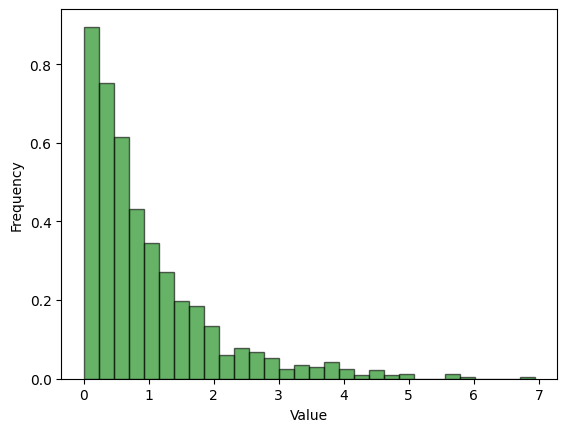
\includegraphics[width=0.5\linewidth]{./Figures/InverseCDF/histogram.png}
	\caption{Histogram of Equation \eqref{fig:inversecdfmethod} with \(\lambda = 1\) applied to \(\mathcal{U}\).}
	\label{fig:inversecdfmethod}
\end{figure}

With this picture, we can see that the histogram of the generated random numbers aligns remarkably well with the target distribution, however, we need to make more trials to be sure. We alredy know the theoreticall mean and variance of the exponential distribution, so we can compare them with the mean of the samples while the number of trials increases. The following Figure~\ref{fig:uniformerrorcdf} and Figure~\ref{fig:exponentialerrorcdf} shows the error to the theoretical mean as the number of trials increases for the uniform and exponential distribution.

\begin{figure}[H]
	\centering
	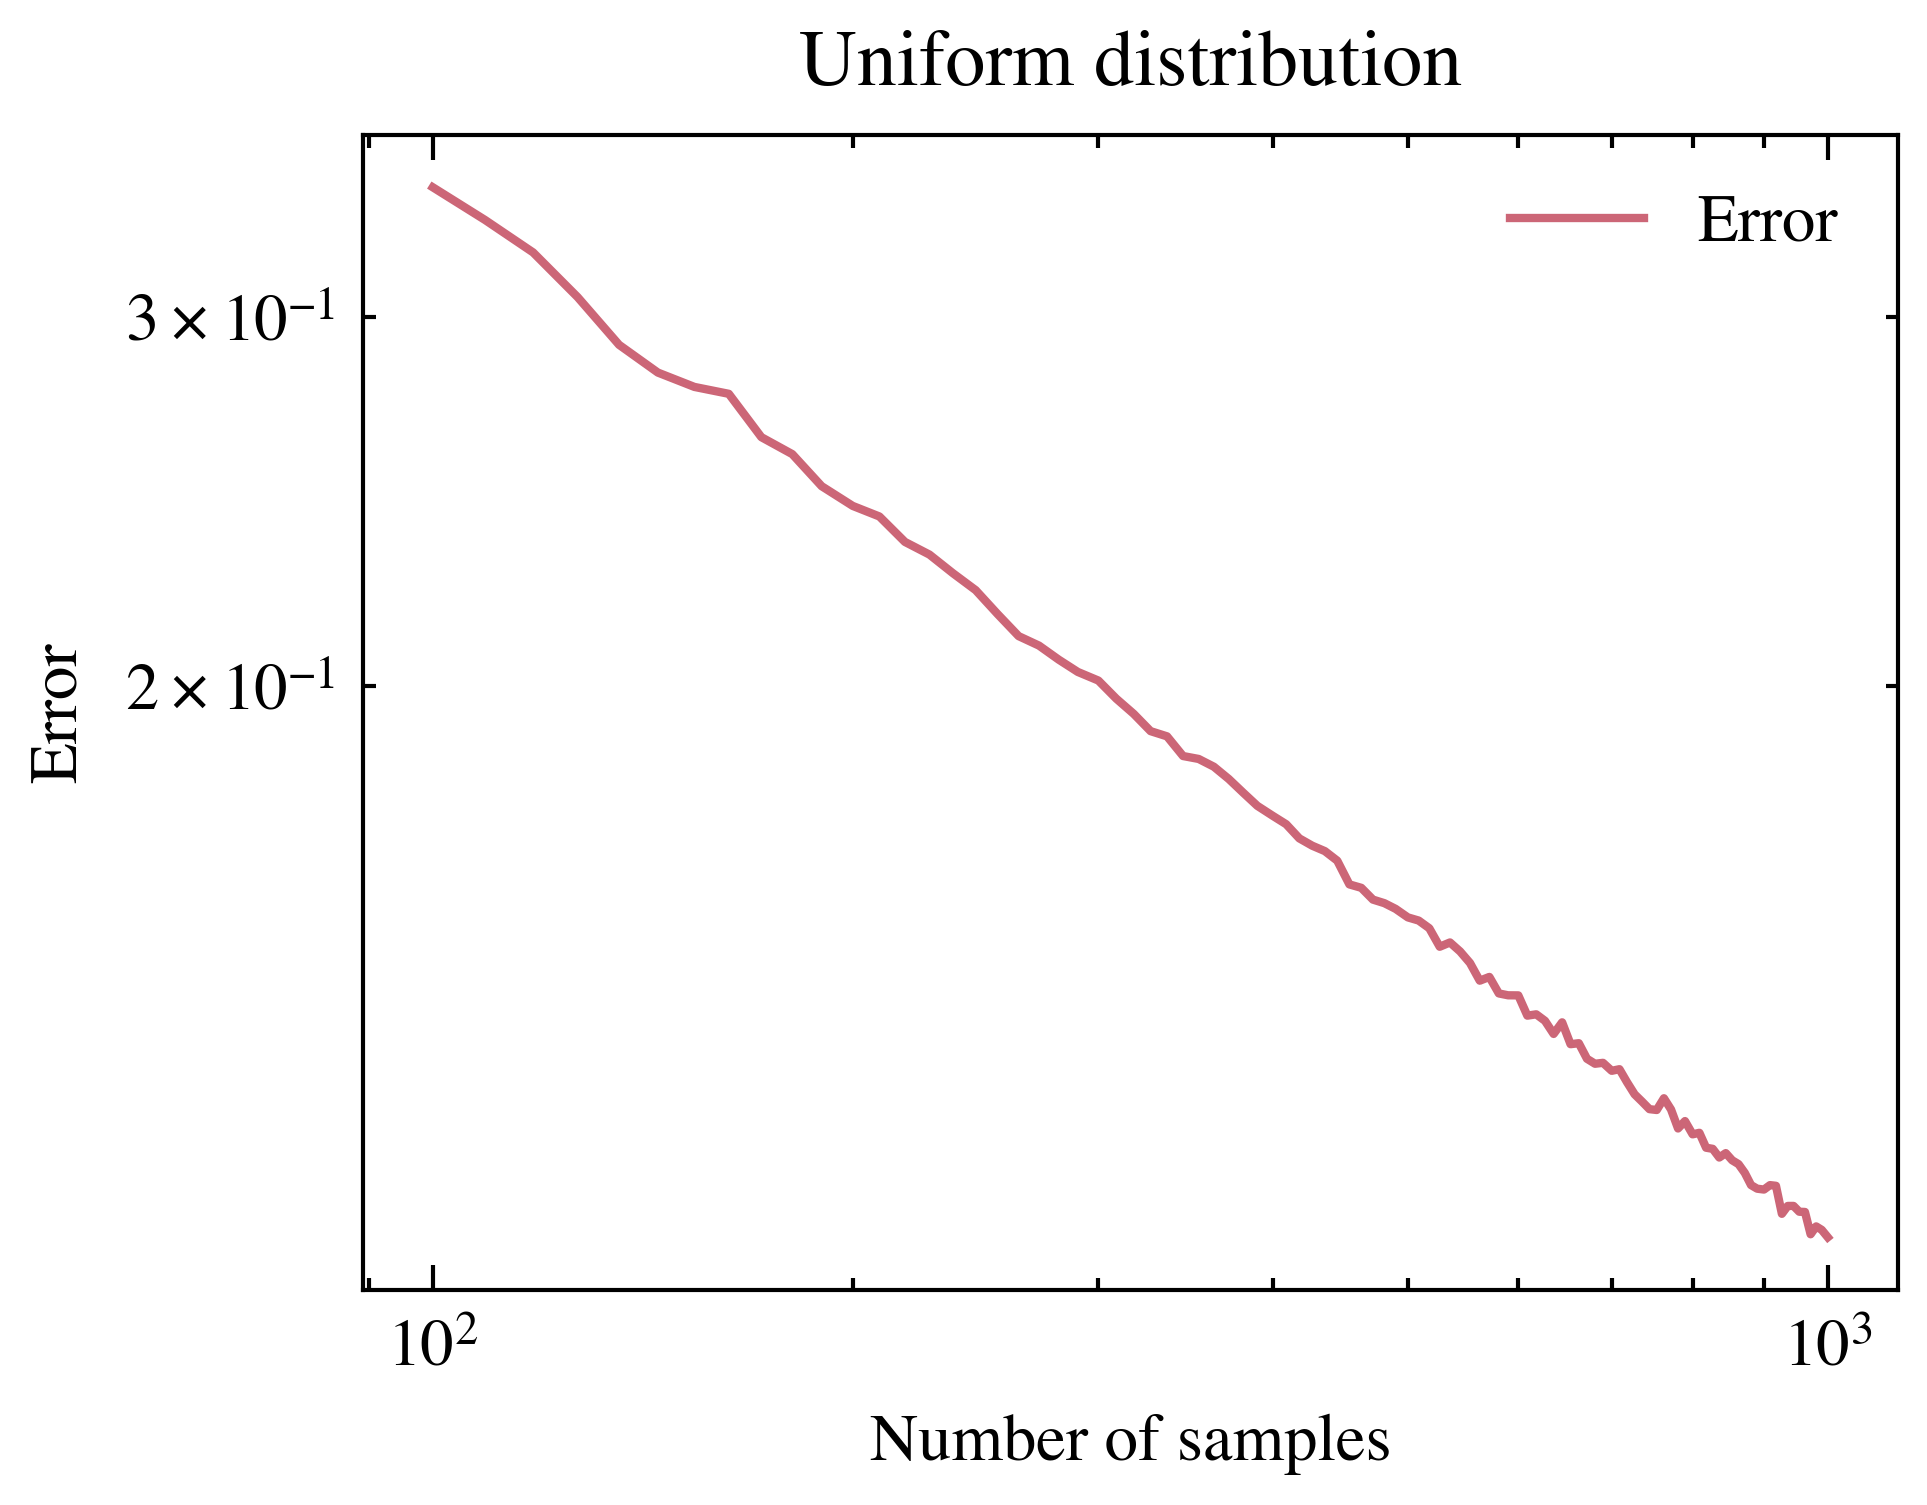
\includegraphics[width=0.5\linewidth]{./Figures/InverseCDF/uniform_error.png}
	\caption{Error to the theoretical mean as the number of trials increases for the uniform distribution}
	\label{fig:uniformerrorcdf}
\end{figure}

\begin{figure}[H]
	\centering
	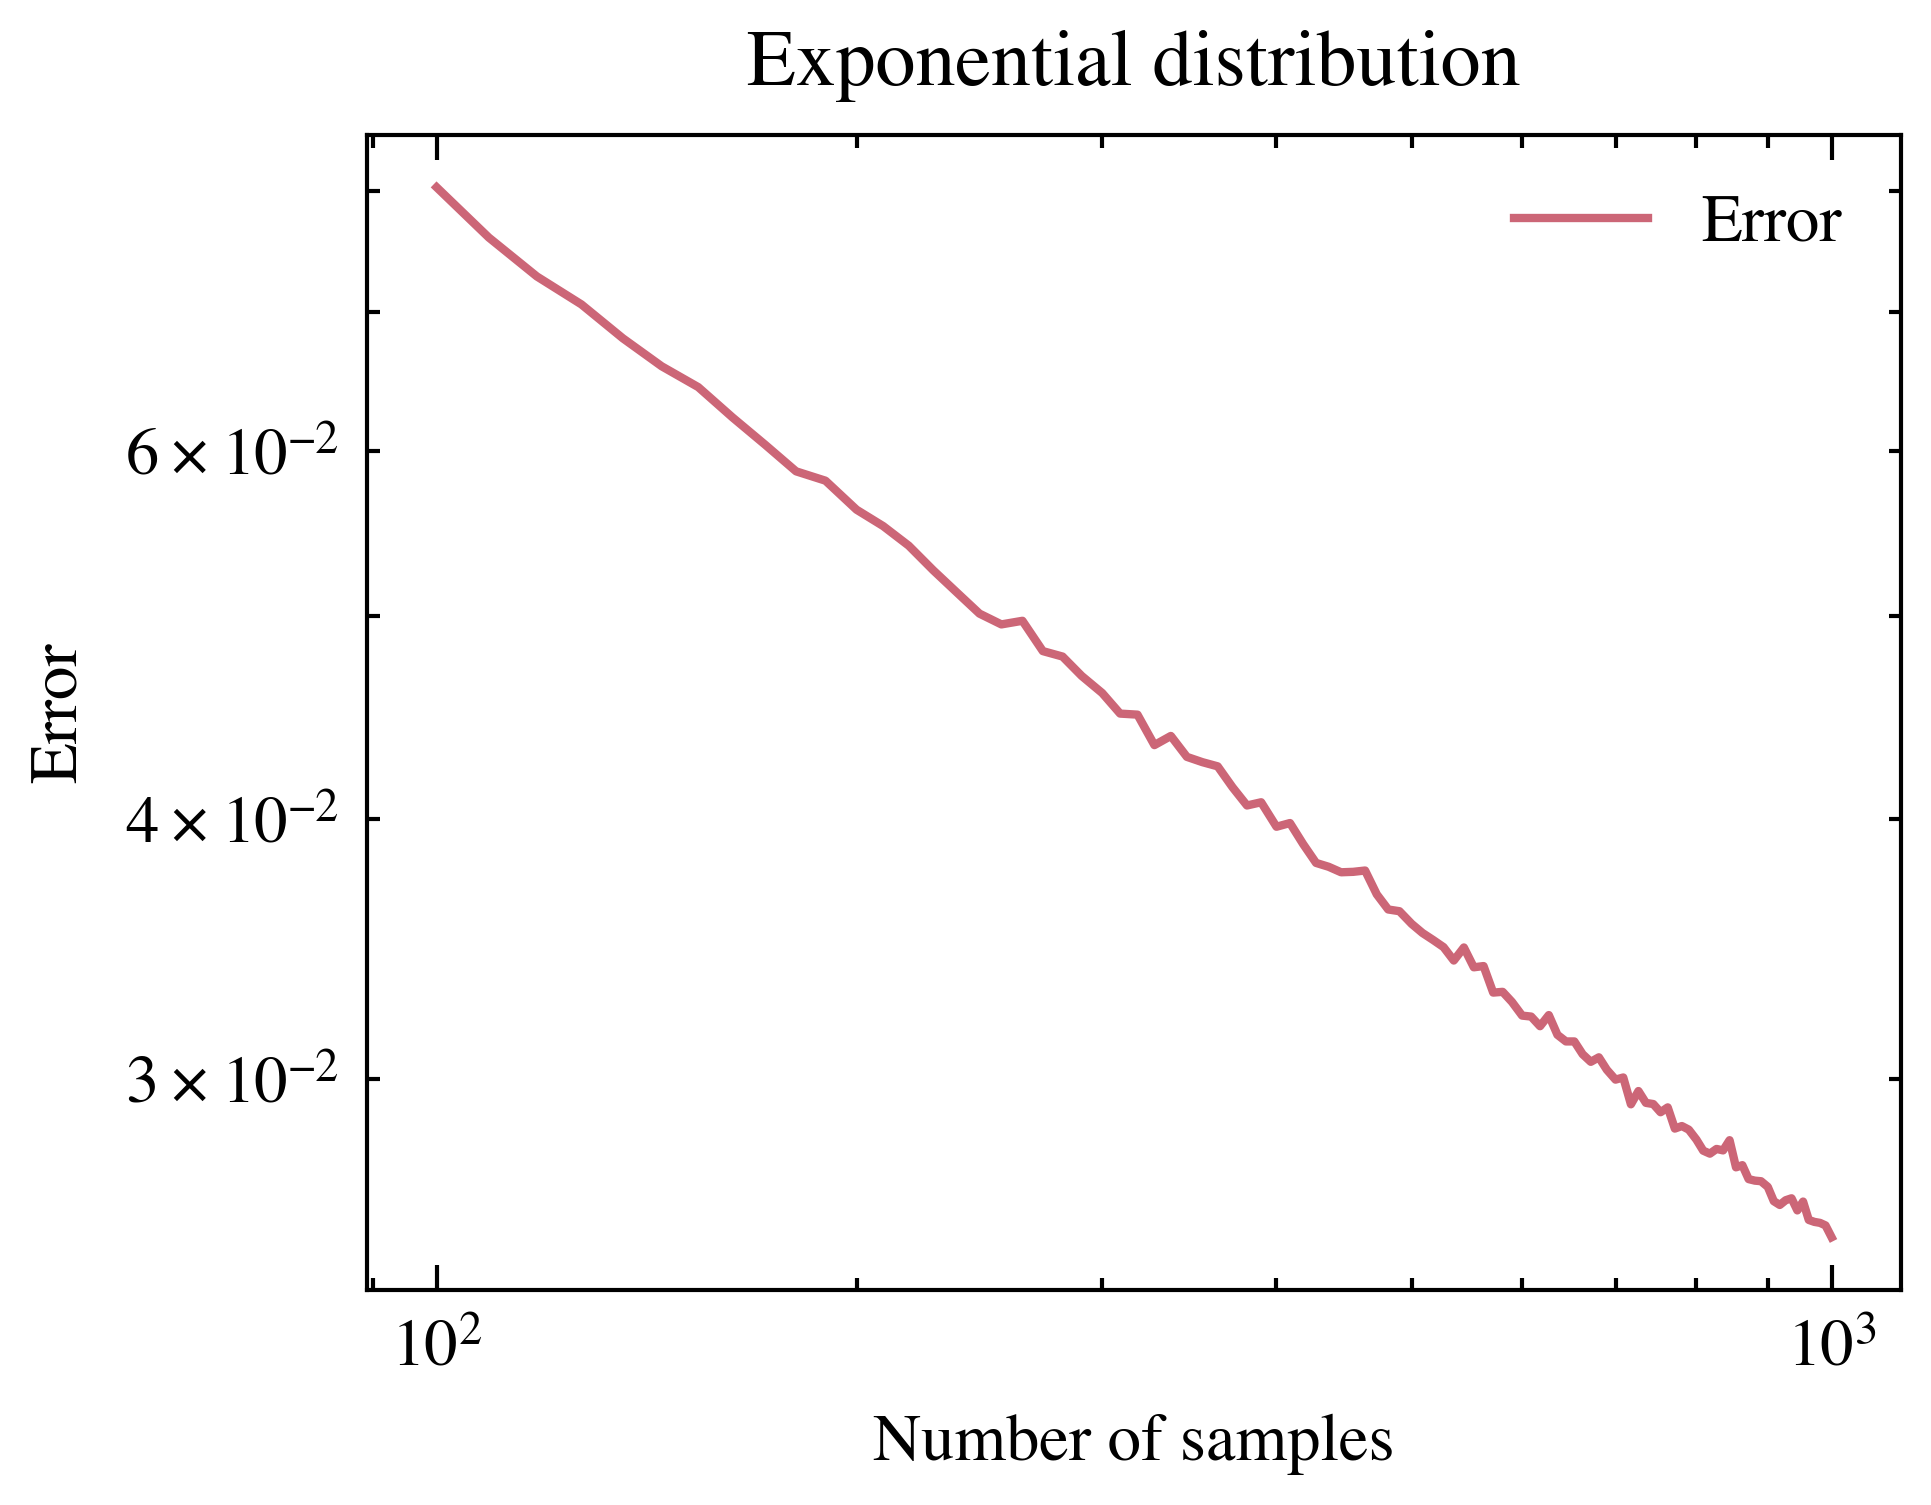
\includegraphics[width=0.5\linewidth]{./Figures/InverseCDF/exponential_error.png}
	\caption{Error to the theoretical mean as the number of trials increases for the exponential distribution}
	\label{fig:exponentialerrorcdf}
\end{figure}

In drawing conclusions from the observed alignment of the histograms of generated random numbers with the target distribution, there appears to be a noteworthy correlation, as evidenced by Figures~\ref{fig:uniformerrorcdf} and~\ref{fig:exponentialerrorcdf}. These figures tentatively suggest a coherence between the theoretical and empirical means, hinting at a plausible reliability of the inverse CDF methods used. The error plots seem to indicate a convergence, providing a preliminary yet cautious optimism about the accuracy of the generated numbers in adhering to the desired distributions.



\subsection{Rejection Sampling method}

The Rejection Sampling method is a method to generate pseudo-random numbers for any probability distribution given its probability density function. The idea is to generate a set of random numbers from a probability distribution that is easy to sample from and then reject the numbers that are not in the desired distribution. The Algorithm~\ref{alg:rejectionalg} is as follows:

\begin{center}
	\begin{minipage}{0.7\linewidth} % Adjust the minipage width to accomodate for the length of algorithm lines
		\begin{algorithm}[H]
			1. Generate a set of random numbers \(X \sim g(x)\) \;
			2. Generate a set of random numbers \(U \sim \mathcal{U}(0,1)\) \;
			3. If \(U \leq \frac{f(X)}{Mg(X)}\) then accept \(X\), otherwise reject \(X\) \;
			\caption{Rejection Sampling mehtod} % Algorithm name
			\label{alg:rejectionalg}   % optional label to refer to
		\end{algorithm}
	\end{minipage}
\end{center}

Being \(g(x)\) the probability density function with which we alredy know how to generate random numbers; \(f(x)\) the target probability density function; and \(M\) a factor we can choose manually and can be optimized.

Let's see this with one example. We want to generate a set of random numbers from the following probability density function: 

\begin{equation} \label{eq:bimodal} f(x) = 0.3e^{-0.2x^2}+0.7e^{-0.2(x-5)^2} \end{equation}

In the other side, we will use the normal distribution as the easy distribution to sample from. So applying the algorithm, we can generate a set of random numbers \(X \sim \mathcal{N}(\mu,\sigma)\) and a set of random numbers \(U \sim \mathcal{U}(0,1)\). Then, we accept the numbers that are in the desired distribution. 

First of all, it is important to note that we have to choose \(\mu\), \(\sigma\) and \(M\) in order to envelope the desired distribution with our normal distribution maximizing the acceptance rate. Since the bimodal distribution is almost between -5 and 10, we can choose \(\mu = 2.5\) and \(\sigma = 3\). Then, to maximize the acceptance rate, we have to envelope the desired distribution but with the minimun space between them as possible, so we should take M with the following formula:

\begin{equation} 
	M = \max_{x \in \mathbb{R}} \frac{f(x)}{g(x)} 
\end{equation}

Being \(g(x)\) the probability density function of the normal distribution and \(f(x)\) the probability density function of the desired distribution. In this case, \(M \approx 2.15\).

The following Figure~\ref{fig:rejectionhist} shows the histogram of the generated random numbers and the probability density function of the desired and the easy distribution.

\begin{figure}[H]
	\centering
	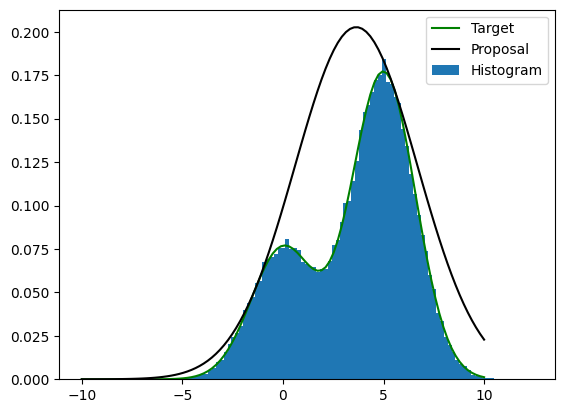
\includegraphics[width=0.5\linewidth]{./Figures/AcceptanceRejection/hist.png}
	\caption{Histogram of the generated random numbers, Equation \eqref{eq:bimodal} and PDF of \(\mathcal{N}(2.5,3)\) scaled by \(M \approx 2.15\).}
	\label{fig:rejectionhist}
\end{figure}

With this picture, we can see that the histogram of the generated random numbers aligns remarkably well with the target distribution, however, we need to make more trials to be sure. As we did in the previous section, we can compare the mean of the samples with the theoretical mean as the number of trials increases. The following Figure~\ref{fig:rejectionerror} shows the error to the theoretical mean. As disclaimer, we know the mean of the function using the following formula: \(\int_{-\infty}^{\infty} xf(x)dx\). However, we can't compute this integral analytically, so we will use the following approximation: \(\frac{1}{n}\sum_{i=1}^{n} x_i\).

\begin{figure}[H]
	\centering
	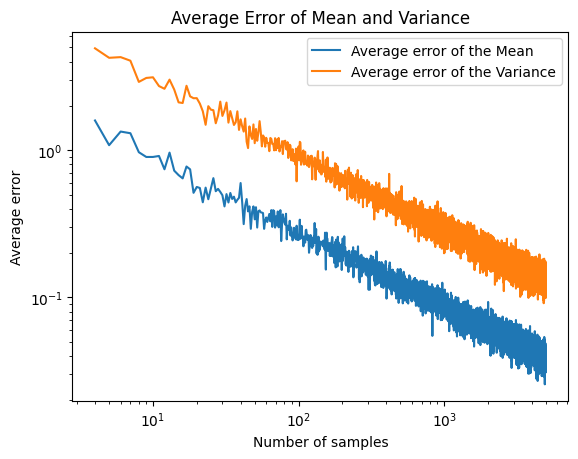
\includegraphics[width=0.5\linewidth]{./Figures/AcceptanceRejection/error_linear_regression.png}
	\caption{Error to the theoretical mean as the number of trials increases}
	\label{fig:rejectionerror}
\end{figure}

In drawing conclusions from the observed alignment of the histograms of generated random numbers with the target distribution, there appears to be a noteworthy correlation, as evidenced by Figure~\ref{fig:rejectionerror}. This figure tentatively suggests a coherence between the theoretical and empirical means, hinting at a plausible reliability of the rejection sampling methods used. The error plot seems to indicate a convergence, providing a preliminary yet cautious optimism about the accuracy of the generated numbers in adhering to the desired distributions.

\subsection{Empirical validation of the Law of Large Numbers}

The Law of Large Numbers posits that, as the number of trials in an experiment increases, the average of the results obtained should converge towards the expected value of the probability distribution in question. Formally, the law can be expressed as follows:

\begin{theorem}[Law of Large Numbers]
 Let \(\{X_1, X_2, ...\}\) be a sequence of independent and identically distributed random variables drawn from a distribution of mean \(\mu\). And let \(\bar{X}_n = \frac{1}{n}\sum_{i=1}^{n} X_i\) be the average of the first \(n\) elements in the sequence. Then, as \(n\) approaches infinity, the random variables \(\bar{X}_n\) converge in probability to \(\mu\):

 \begin{equation}
	 \bar{X}_n \rightarrow \mu \ \ as \ n \rightarrow \infty
\end{equation}

\end{theorem}

Given our established ability to generate random numbers reflecting specific probability distributions, we can select a distribution, generate a set of numbers corresponding to it, and then contrast the calculated averages and means of the target distribution while escalating the number of trials. To illustrate, employing the normal distribution with a mean of 0 provides the results depicted in Figure~\ref{fig:verificationlln}.

\begin{figure}[H]
	\centering
	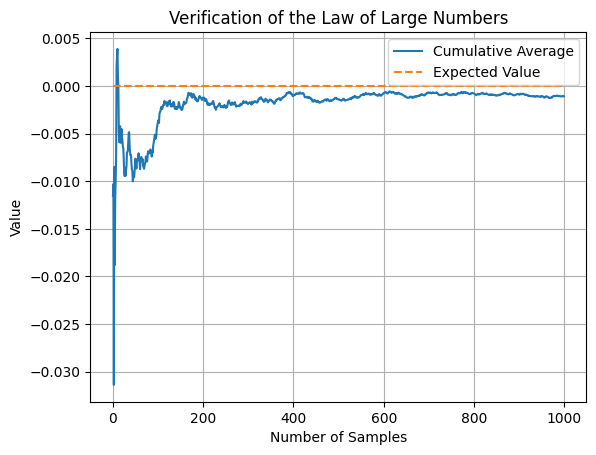
\includegraphics[width=0.5\linewidth]{./Figures/LLN/verif.png}
	\caption{Comparison of the method's average with the mean of the normal distribution (0)}
	\label{fig:verificationlln}
\end{figure}

Refining Figure~\ref{fig:verificationlln} to display the absolute error in relation to the mean, and plotting it on a logarithmic scale, yields Figure~\ref{fig:verificationllnlog}.

\begin{figure}[H]
	\centering
	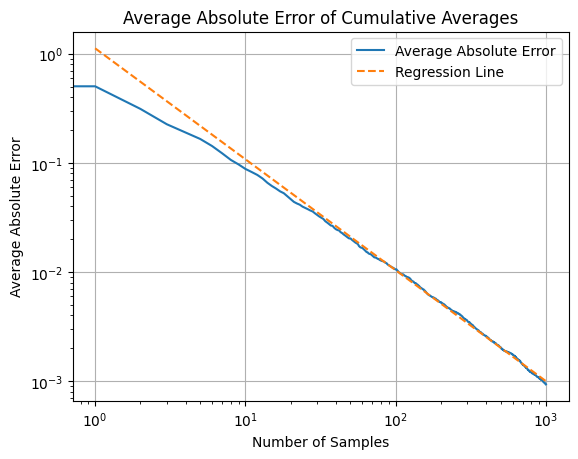
\includegraphics[width=0.5\linewidth]{./Figures/LLN/verifloglog.png}
	\caption{Logarithmic depiction of the absolute error relative to the mean}
	\label{fig:verificationllnlog}
\end{figure}

The visual representation in Figure~\ref{fig:verificationllnlog} substantiates that the error indeed diminishes as the number of trials augments, validating the assertion of the Law of Large Numbers that the experimental mean approaches the theoretical mean with an increasing number of observations.

\subsection{Empirical Validation of the Central Limit Theorem}

The Central Limit Theorem (CLT) posits a pivotal foundational theorem in probability theory, signifying that, irrespective of the shape of the original distribution, the distribution of sample means will approximate a normal distribution as the sample size burgeons. To empirically validate this theorem, we can simulate a series of random numbers from any given probability distribution and systematically calculate their mean. By perpetuating this process, we can construct a histogram of the means and scrutinize whether it converges to a normal distribution, aligning with the theorem's prediction. Formally, the theorem can be expressed as follows:

\begin{theorem}[Lindeberg–Lévy CLT]
	Suppose \(\{X_1, X_2, ..., X_n\}\) is a sequence of independent and identically distributed random variables drawn from a distribution of mean \(\mathbb{E}(X_i) = \mu\) and finite variance \(\mathbb{V}(X_i) = \sigma^2\). Then, as \(n\) approaches infinity, the random variables \(\sqrt{n}(\bar{X}_n - \mu)\) converge in distribution to a normal \(\mathcal{N}(0, \sigma^2)\):

	\begin{equation}
		\sqrt{n}(\bar{X}_n - \mu) \xrightarrow{d} \mathcal{N}(0, \sigma^2)
	\end{equation}
\end{theorem}

For illustrative purposes, consider the uniform distribution, which yields a histogram as delineated in Figure~\ref{fig:verificationclt}.

\begin{figure}[H]
	\centering
	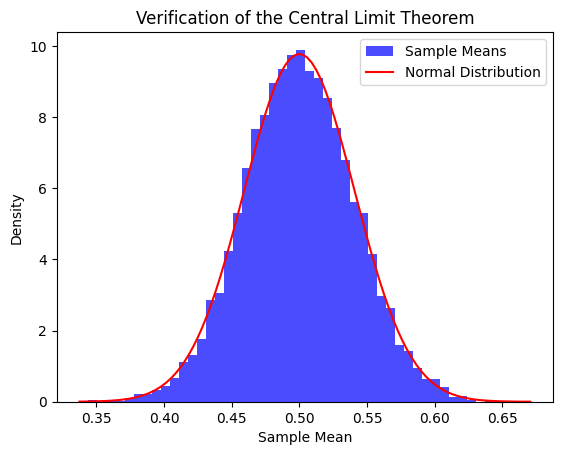
\includegraphics[width=0.5\linewidth]{./Figures/CLT/verif.png}
	\caption{Histogram illustrating the convergence of the means of the uniform distribution}
	\label{fig:verificationclt}
\end{figure}

In congruence with the methodology espoused in previous sections, we have juxtaposed the empirical mean of the samples with the theoretical mean, progressively augmenting the number of trials. Figure~\ref{fig:meanerror} delineates the deviation from the theoretical mean, and Figure~\ref{fig:varianceerror} represents the deviation from the theoretical variance, both as functions of the number of trials.

\begin{figure}[H]
	\centering
	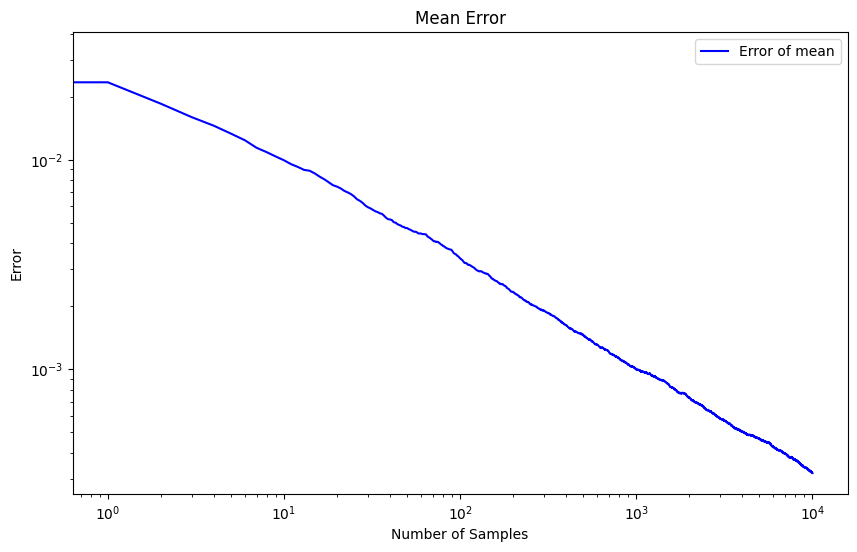
\includegraphics[width=0.5\linewidth]{./Figures/CLT/meanerror.png}
	\caption{Deviation from the theoretical mean as a function of the number of trials}
	\label{fig:meanerror}
\end{figure}

\begin{figure}[H]
	\centering
	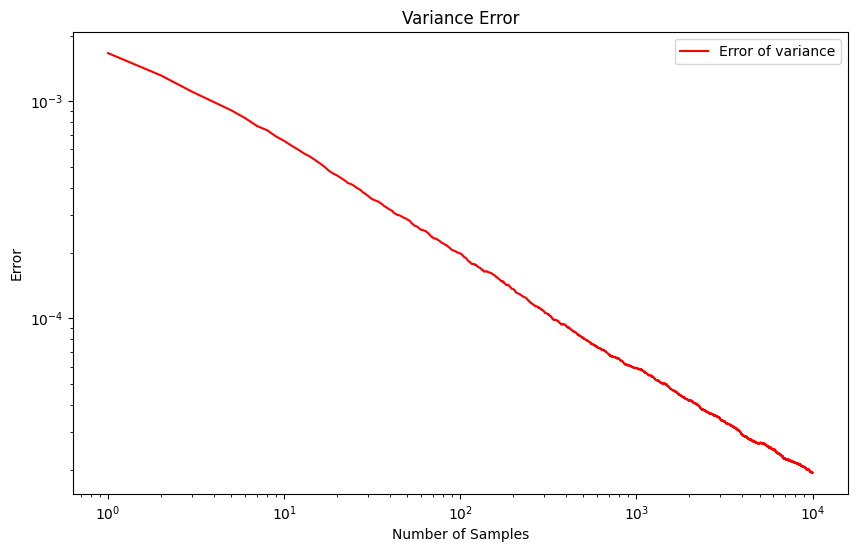
\includegraphics[width=0.5\linewidth]{./Figures/CLT/varianceerror.png}
	\caption{Deviation from the theoretical variance as a function of the number of trials}
	\label{fig:varianceerror}
\end{figure}

A discernible insight gleaned from Figure~\ref{fig:meanerror} and Figure~\ref{fig:varianceerror} is the palpable decrement in deviations from the theoretical values as the trials proliferate. This phenomenological observation substantiates the assertions of the Central Limit Theorem, illuminating the convergence of the distribution of sample means to a normal distribution as the sample size escalates, validating the theoretical underpinnings of the theorem through empirical exploration.

\subsection{Variance reduction techniques}

In the theory of Monte Carlo methods, variance reduction techniques are a pivotal tool to increase the precision of the estimates of the expected value of a random variable. In this section, we will focus on three techniques: Control variates, Importance sampling and Antithetic variates. Also, we will introduce an example problem in which we will apply these techniques to compare them.

First of all, let introduce the variance reduction formally. Let \(\{X_1, X_2, ..., X_n\}\) be a sequence of independent and identically distributed random variables drawn from a distribution of mean \(\mathbb{E}(X_i) = \mu\) and finite variance \(\mathbb{V}(X_i) = \sigma^2\). Then, the expected value of a random variable is defined as follows:

\begin{equation} 
	\label{eq:expectedvalueestimate} 
	\hat{\mathbb{E}}(X) = \frac{1}{n} \sum_{i=1}^{n} X_i
\end{equation}

So, we want to make zero the variance of our estimation. Since the variance is defined as follows:

\begin{equation} 
	\label{eq:variance} 
	Var(\hat{\mathbb{E}}(X)) = \frac{Var(X)}{n}
\end{equation}

Consequently, we are presented with two avenues for optimization: increasing the value of \(n\), or diminishing the variance of \(\mathbb{E}\). Assuming that \(n\) is predetermined and unalterable, our focus would then shift to minimizing the variance of \(X\).

Since we are going to introduce and compare the three techniques, first of all we need to introduce the problem we are going to solve. The problem is that we want to estimate the following integral:

\begin{equation} \label{eq:integralvariancereduction} I = \int_{0}^{1} x^2 \ dx \end{equation}

It should be noted that the selection of the integral for this demonstration was intentional; a readily solvable integral was chosen for its ease of analytical computation, allowing for a straightforward comparison with theoretical values. Nonetheless, the methods illustrated herein are equally applicable and potent for evaluating integrals that pose substantial challenges to analytical computation.

\subsubsection{Preliminaries}

First of all we have to compute which is the estimation we alredy can have without applying any variance reduction technique. We can compute the integral analytically. We know that the mean of the variable in a probability space is defined as follows:

\begin{equation} 
	\label{eq:directmethod} 
	\mathbb{E}(g(X)) = \int_b^a g(x)f(x) \ dx
\end{equation}

Since \(p(x) = \frac{1}{b-a}\) for the uniform distribution, we can apply Equation \eqref{eq:directmethod} to Equation \eqref{eq:integralvariancereduction} and we obtain:

\begin{equation} \label{eq:directmethodintegral} I = \int_{0}^{1} x^2 \ dx = \mathbb{E}(g(X)) = \int_0^1 x^2 \frac{1}{1-0} \ dx = \frac{1}{3} \end{equation}

So, we only have to generate a set of random numbers \(X \sim \mathcal{U}(0,1)\), apply \(f(x) = x^2\) and get the mean of the sample which is the estimate of the integral. The following Figure~\ref{fig:directmethod} shows the error to the theoretical value as the number of trials increases.

\begin{figure}[H]
	\centering
	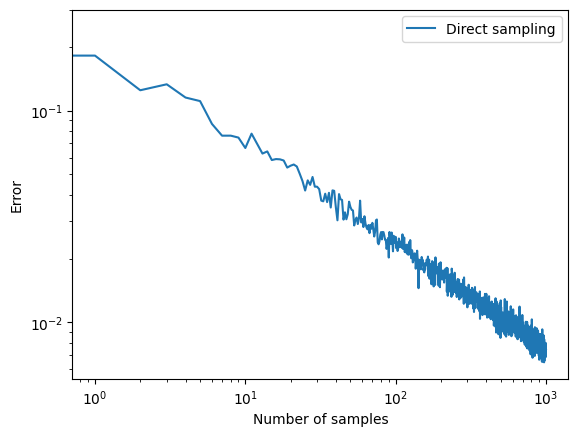
\includegraphics[width=0.5\linewidth]{./Figures/VarianceReduction/direct.png}
	\caption{Error to the theoretical value as the number of trials increases using the direct method}
	\label{fig:directmethod}
\end{figure}

\subsubsection{Control variates}

Control variates is a variance reduction technique with the following idea: Let \(\mu\) the parameter we want to estimate, and assume we have a statistic \(Y\) such that \(\mathbb{E}(Y) = \tau\). Then, we can estimate \(\mu\) by estimating \(\mathbb{E}(Y)\) as \(\hat{\mathbb{E}}(Y)\) and correcting the bias with the following formula:

\begin{equation} \label{eq:controlvariates} \hat{\mu} = \mu + c(\tau - \hat{\mathbb{E}}(Y)) \end{equation}

Being \(c\) a constant which minimize the variance of the estimation. It is computed as follows:

\begin{equation} 
	\label{eq:controlvariatesconstant} 
	c = -\frac{Cov(X,Y)}{Var(Y)} 
\end{equation}

In our case, we can use the knowledge of the mean of the uniform distribution to correct the bias, so in each iteration we can compute the mean of the sample of random numbers of \(\mathcal{U}(0,1)\), and knowing that the mean of the uniform distirbution is \(0.5\) we can apply Equation \eqref{eq:controlvariates} to obtain the estimate of the integral. The following Figure~\ref{fig:controlvariates} shows the error to the theoretical value as the number of trials increases.

\begin{figure}[H]
	\centering
	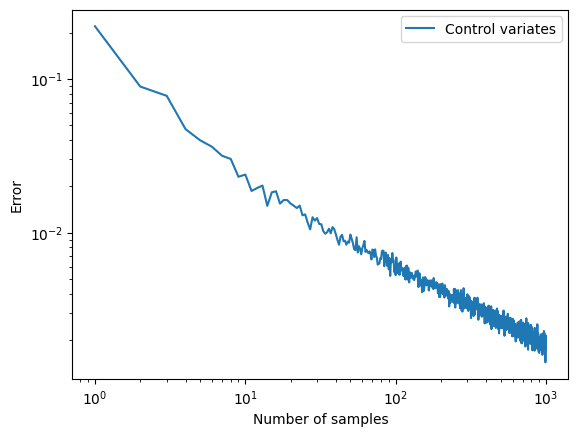
\includegraphics[width=0.5\linewidth]{./Figures/VarianceReduction/control.png}
	\caption{Error to the theoretical value as the number of trials increases using the control variates method}
	\label{fig:controlvariates}
\end{figure}

\subsubsection{Importance sampling}

Importance sampling is another variance reduction technique. Instead of using the knowledge of another estimator to reduce the bias of our sample, as done in the control variates method, in this case the idea is using the knowledge of the actual function we want to integrate, so instead of using a uniform distribution, we can use another distribution that is more similar to the function we want to integrate, in order to try more samples in the areas where the function is more important. 

In our example, we know that the function is a parabola, so instead of using a sample which follows an uniform distribution, maybe we can use a distribution that fits better with the shape of the function. In this case, we have chosen \(Beta(2.9,1)\). In order to illustrate this, in the following Figure~\ref{fig:beta42_f} we can see the function we want to integrate, the PDF of \(Beta(2.9,1)\) and the PDF of \(\mathcal{U}(0,1)\).

\begin{figure}[H]
	\centering
	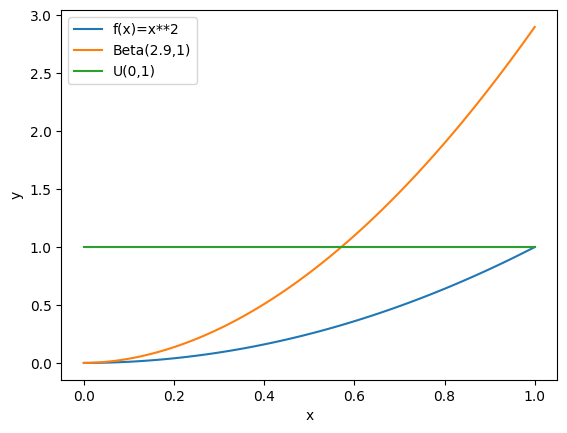
\includegraphics[width=0.5\linewidth]{./Figures/VarianceReduction/beta.png}
	\caption{Function we want to integrate, PDF of \(Beta(2.9,1)\) and PDF of \(\mathcal{U}(0,1)\)}
	\label{fig:beta42_f}
\end{figure}

As we can see, the PDF of \(Beta(2.9,1)\) fits better with the shape of the function we want to integrate, so we can expect that the error will decrease faster than the direct method and the control variates method. 

So the idea is to generate a sample of random numbers \(X \sim Beta(2.9,1)\), and take \(Y = \frac{f(X)}{g(X)}\) as the estimator of the integral, being \(f(x) = x^2\) and \(g(x)\) the PDF of \(Beta(2.9,1)\). The following Figure~\ref{fig:importancesampling} shows the error to the theoretical value as the number of trials increases.

\begin{figure}[H]
	\centering
	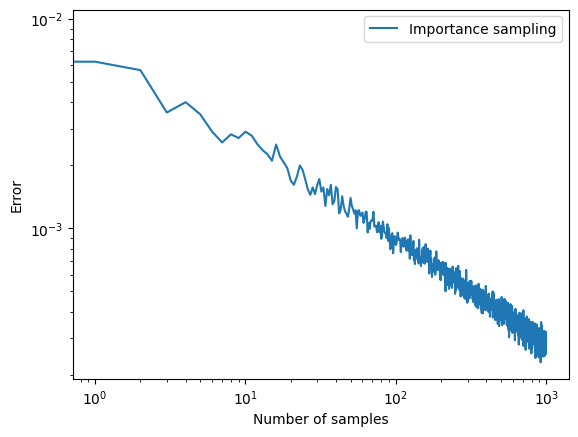
\includegraphics[width=0.5\linewidth]{./Figures/VarianceReduction/importance.png}
	\caption{Error to the theoretical value as the number of trials increases using the importance sampling method}
	\label{fig:importancesampling}
\end{figure}

\subsubsection{Stratified sampling}

The idea is to divide the interval of the stratified sampling is pretty simple. We divide the interval in \(n\) subintervals, and we generate a sample of random numbers for each subinterval. Doing this, we are trying to reduce the variance of the mean of the distribution we are considering, so the sample is more representative of the distribution. The following Figure~\ref{fig:stratifiedsampling} shows the error to the theoretical value as the number of trials increases.

\begin{figure}[H]
	\centering
	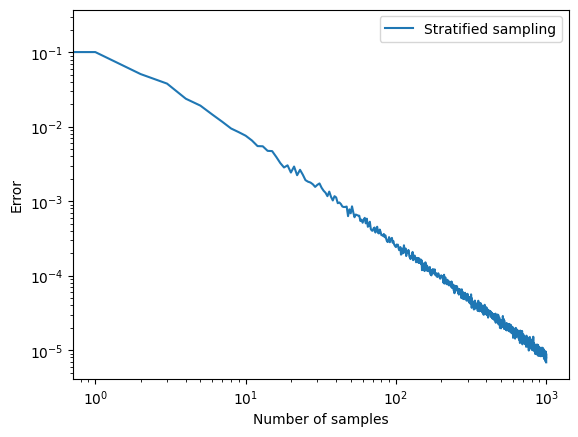
\includegraphics[width=0.5\linewidth]{./Figures/VarianceReduction/stratified.png}
	\caption{Error to the theoretical value as the number of trials increases using the stratified sampling method}
	\label{fig:stratifiedsampling}
\end{figure}

\subsubsection{Antithetic variates}

The Antithetic variates method consists on taking for each random sample, its antithetic, i.e. the symmetric with respect to the mean of the distribution. The idea is that the variance of the mean of the distribution is reduced, since the mean of the antithetic is the same as the mean of the distribution. In our case, we have generated a sample \(\mathcal{U} \sim \mathcal{U}(0,0.5)\) and its antithetic \(mathcal{U}' = \{1 - x \ : \ x \in mathcal{U}\}\). Taking \(X = \mathcal{U} \bigcup \mathcal{U}' \), we can apply Equation \eqref{eq:expectedvalueestimate} to \(f(X)\) to obtain the estimate of the integral. The following Figure~\ref{fig:antitheticvariates} shows the error to the theoretical value as the number of trials increases.

\begin{figure}[H]
	\centering
	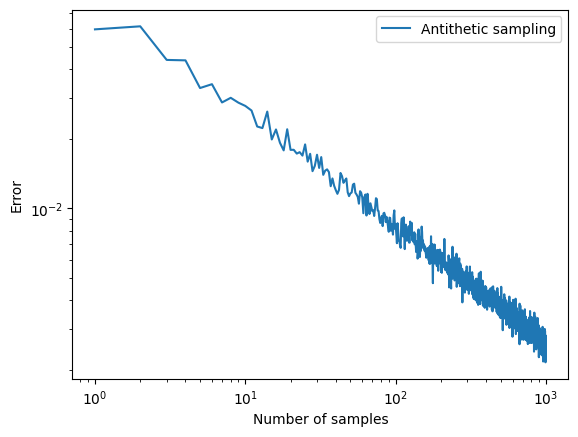
\includegraphics[width=0.5\linewidth]{./Figures/VarianceReduction/antithetic.png}
	\caption{Error to the theoretical value as the number of trials increases using the antithetic variates method}
	\label{fig:antitheticvariates}
\end{figure}

\subsubsection{Comparative Review}

After unraveled the intricacies of each method and confirming the convergence of each approach described in this study, we now turn to a more focused comparison of these techniques. The goal is simple: find out which method works best for our specific problem. See Figure~\ref{fig:comparisonvariancereduction} for a visual representation of the error in relation to the theoretical value as we increase the number of trials for each method.

\begin{figure}[H]
\centering
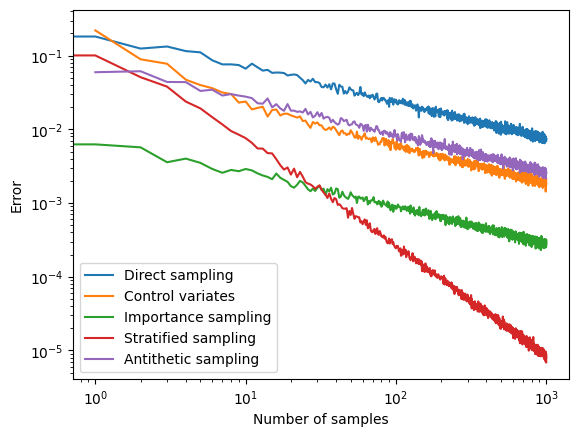
\includegraphics[width=0.5\linewidth]{./Figures/VarianceReduction/comparison.png}
\caption{Error variation with increased trials for each method.}
\label{fig:comparisonvariancereduction}
\end{figure}

Looking at the data, it’s clear that stratified sampling takes the lead with its quicker convergence compared to the other methods. However, claiming it as the undisputed champion would be premature, especially when we’ve explored just one problem. To firm up this initial finding, we need to dig deeper and explore a variety of problems.

Next, we'll broaden our investigation to a more complex problem, applying the methods we’ve discussed to estimate the following integrals:

\begin{equation} 
	\label{eq:integralvariancereduction1} 
	Parabola = \int_{0}^{1} x^2 \ dx 
\end{equation}

\begin{equation} 
	\label{eq:integralvariancereduction2} 
	Gaussian = \int_{0}^{1} e^{-x^2} \ dx
\end{equation}

\begin{equation} 
	\label{eq:integralvariancereduction3} 
	Sine = \int_{0}^{1} \sin(x) \ dx
\end{equation}

\begin{equation} 
	\label{eq:integralvariancereduction4} 
	Polynomial = \int_{0}^{1} x^3 - 2x^2 + x \ dx
\end{equation}

\begin{equation} 
	\label{eq:integralvariancereduction5} 
	Exponential = \int_{0}^{1} e^x \ dx
\end{equation}

Using these examples, we can now draw comparisons between the methods in a broader context. Figure~\ref{fig:comparisonvariancereduction2} illustrates the error of each method applied to each function.

\begin{figure}[H]
\centering
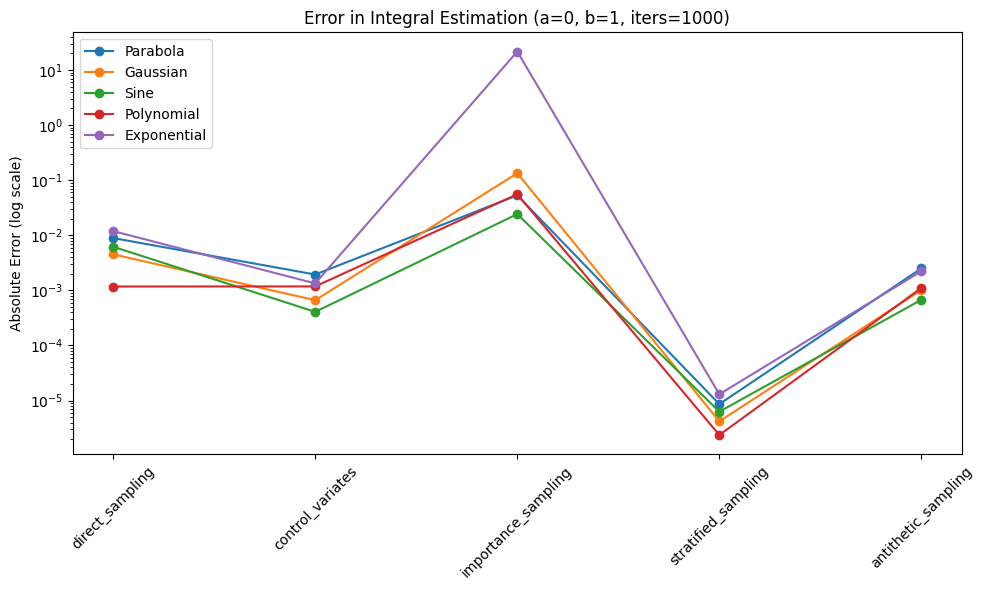
\includegraphics[width=0.5\linewidth]{./Figures/VarianceReduction/comparisonintegrals.png}
\caption{Method-wise error in each function.}
\label{fig:comparisonvariancereduction2}
\end{figure}

Notably, for the importance sampling method, we opted for a normal distribution with the mean and variance of each function to maintain fairness in comparison, avoiding manual distribution selection for every function.

Reviewing the data, stratified sampling again stands out for its rapid convergence. However, the importance sampling lags, a likely outcome of applying a general normal distribution for all functions, each requiring a unique distribution. But to outrightly conclude that stratified sampling is the go-to method would be a rush to judgment, given our exploration is based on limited scenarios. Thorough exploration involving varied problems is essential to cement our initial conclusions while maintaining the professional and scientific rigor of our exploration.



\end{document}
